\documentclass[10pt]{beamer}
\usetheme[
%%% options passed to the outer theme
%    hidetitle,           % hide the (short) title in the sidebar
%    hideauthor,          % hide the (short) author in the sidebar
%    hideinstitute,       % hide the (short) institute in the bottom of the sidebar
%    shownavsym,          % show the navigation symbols
%    width=2cm,           % width of the sidebar (default is 2 cm)
%    hideothersubsections,% hide all subsections but the subsections in the current section
%    hideallsubsections,  % hide all subsections
    left,               % right of left position of sidebar (default is right)
%%% options passed to the color theme
%    lightheaderbg,       % use a light header background
  ]{AAUsidebar}

% If you want to change the colors of the various elements in the theme, edit and uncomment the following lines
% Change the bar and sidebar colors:
%\setbeamercolor{AAUsidebar}{fg=red!20,bg=red}
%\setbeamercolor{sidebar}{bg=red!20}
% Change the color of the structural elements:
%\setbeamercolor{structure}{fg=red}
% Change the frame title text color:
%\setbeamercolor{frametitle}{fg=blue}
% Change the normal text color background:
%\setbeamercolor{normal text}{bg=gray!10}
% ... and you can of course change a lot more - see the beamer user manual.


\usepackage[utf8]{inputenc}
\usepackage[english]{babel}
\usepackage[T1]{fontenc}
\usepackage{multimedia}
\usepackage{graphicx} % enable fitting figures
\usepackage{wrapfig}
\usepackage{adjustbox}
% Or whatever. Note that the encoding and the font should match. If T1
% does not look nice, try deleting the line with the fontenc.
\usepackage{helvet}
\usepackage{tikz}
\usetikzlibrary{shapes,shapes.geometric, arrows,positioning,calc}
\tikzset{
	block/.style = {draw, fill=white, rectangle, minimum height=3em, minimum width=3em},
	tmp/.style  = {coordinate}, 
	sum/.style= {draw, fill=white, circle, node distance=1cm},
	input/.style = {coordinate},
	output/.style= {coordinate},
	pinstyle/.style = {pin edge={to-,thin,black}
	}
}

\usepackage{amsmath}
\usepackage{amssymb}
\usepackage{kbordermatrix}


% More clever references. 
% Can be \hyperref[sec:intro]{this section}
\usepackage[]{hyperref}
\usepackage{cleveref}

% Set colors of links, cites, urls and such
\hypersetup{
	colorlinks,
	%linkcolor={red!50!black},
	linkcolor={blue!50!black},
	citecolor={blue!50!black},
	urlcolor={blue!80!black}
}

\usepackage{subfig}




% colored hyperlinks
\newcommand{\chref}[2]{%
  \href{#1}{{\usebeamercolor[bg]{AAUsidebar}#2}}%
}

\title[Speed Control and Fore-aft Motion Damping of Floating Wind Turbine]% optional, use only with long paper titles
{Speed Control and Fore-aft Motion Damping of Floating Wind Turbine}

% \subtitle{}  % could also be a conference name

\date{\today}

\author[Martin H. Therkildsen] % optional, use only with lots of authors
{
  Martin H. Therkildsen
}
% - Give the names in the same order as they appear in the paper.
% - Use the \inst{?} command only if the authors have different
%   affiliation. See the beamer manual for an example

\institute[
%  {\includegraphics[scale=0.2]{aau_segl}}\\ %insert a company, department or university logo
  Control and Automation\\
  Aalborg University\\
  Denmark
] % optional - is placed in the bottom of the sidebar on every slide
{% is placed on the title page
  Control and Automation\\
  Aalborg University\\
  Denmark
  
  %there must be an empty line above this line - otherwise some unwanted space is added between the university and the country (I do not know why;( )
}


% specify a logo on the titlepage (you can specify additional logos an include them in 
% institute command below
\pgfdeclareimage[height=1.5cm]{titlepagelogo}{AAUgraphics/aau_logo_new} % placed on the title page
%\pgfdeclareimage[height=1.5cm]{titlepagelogo2}{graphics/aau_logo_new} % placed on the title page
\titlegraphic{% is placed on the bottom of the title page
  \pgfuseimage{titlepagelogo}
%  \hspace{1cm}\pgfuseimage{titlepagelogo2}
}


\begin{document}
% the titlepage
{\aauwavesbg%
\begin{frame}[plain,noframenumbering] % the plain option removes the sidebar and header from the title page
  \titlepage
\end{frame}}


%%%%%%%%%%%%%%%%

% TOC
\begin{frame}{Agenda}{}
\tableofcontents
\end{frame}






% ======================================================================
% Inputs for topics here!

\section{Introduction}
\begin{frame}{Introduction}{What is a wind turbine?}
 		\begin{columns}
 		\begin{column}{.5\textwidth}
 			\textbf{Wind Turbine}
	 			\begin{itemize}
		 			\item Take wind
		 			\item Rotate
		 			\item = Energy			
		 		\end{itemize} \bigskip\bigskip
 			\textbf{Role} 
		 		\begin{itemize}
		 			\item Critical link in Energy and stuff?		
		 		\end{itemize}
 		\end{column}
 	\end{columns}	
\end{frame}

%%%%%%%%%%%%%%%%

\begin{frame}{Introduction}{More intro here?}
	\begin{itemize}
		\item A text
	\end{itemize}\bigskip
\end{frame}


%%%%%%%%%%%%%%%%%%
%\begin{frame}{Big header}{Smaller header}
%	\textbf{Some text}
%	\begin{itemize}
%		\item Item
%	\end{itemize}
%\end{frame}
%


\section{Theoretical Background}

\begin{frame}{Theoretical Background}{Basic aerodynamics and airfoil theory}
	1D momentum theory:
	\begin{itemize}
		\item Air slows down due to delivery of energy from air to rotor blades
		\item Air expands due to conservation of mass
	\end{itemize}

	\begin{figure}[ht]
		\centering
		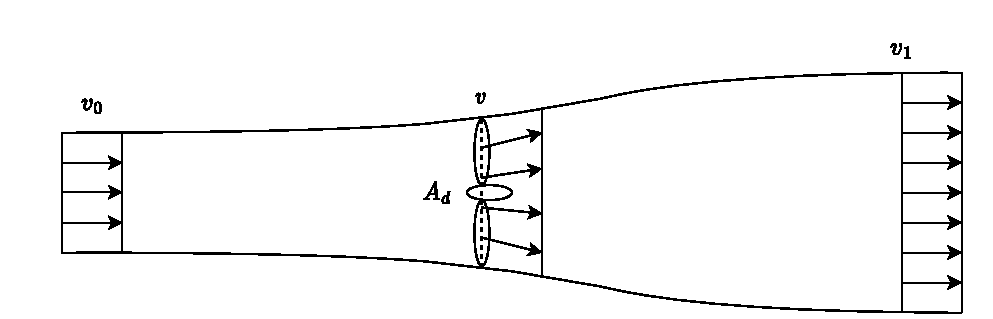
\includegraphics[width=1\linewidth]{../Graphics/FlowThroughRotor.pdf}
		\label{fig:betz}
	\end{figure}
\end{frame}

%%%%%%%%%%%%%%%%%%

\begin{frame}{Theoretical Background}{Basic aerodynamics and airfoil theory}
	Power of wind moving through rotor:
	\begin{equation} \label{eq:power}
		P_{air} = \dfrac{1}{2} \dot{m} \, v_0^2 = \dfrac{1}{2}\rho \, A_d v_0^3
	\end{equation}
	
	Extractable power defined by \textit{power coefficient} $ C_p $:
	\begin{equation}\label{eq:power_w_Cp}
		P_{T} = \dfrac{1}{2} \rho \, A_d v_0^3 C_p(\theta, \lambda)
	\end{equation}
	where $ \lambda $ is the tip-speed ratio (TSR):
	\begin{equation}\label{key}
		\lambda = \dfrac{R \Omega}{v_0}
	\end{equation}
	The theoretically highest achievable $ C_p $ is the \textit{betz limit}:
	\begin{equation}\label{eq:betzlimit}
		C_{pbetz} = 0.5962
	\end{equation}
	The optimal $ C_p $ for a given turbine is achieved at specific TSR and $ \theta $:
	\begin{equation}\label{eq:cp_optimal}
		C_p^\star = C_p(\theta^\star, \lambda^\star)
	\end{equation}
\end{frame}

%%%%%%%%%%%%%%%%%%

\begin{frame}{Theoretical Background}{Blade element theory}
	\begin{itemize}
		\item Forces are calculated on blade sections (b)
		\item Thrust and torque calculated from velocity triangle (a)
	\end{itemize}
	
	\begin{figure}[ht]
		\centering
		\subfloat[Blade cross section]{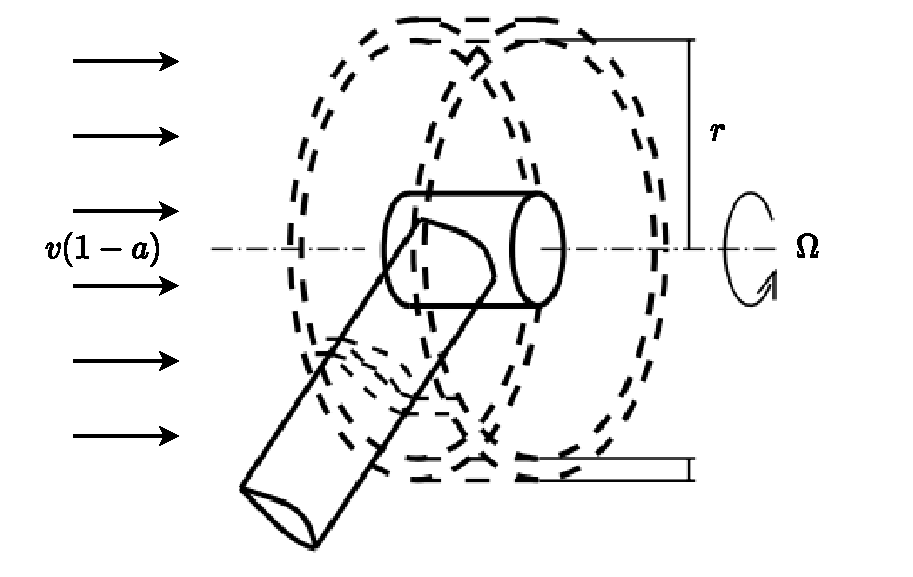
\includegraphics[width=.44\textwidth]{../Graphics/RotorBladeElement.pdf}%
			\label{fig:blade_vel_triangles}}
		\hfil
		\subfloat[Velocity triangle]{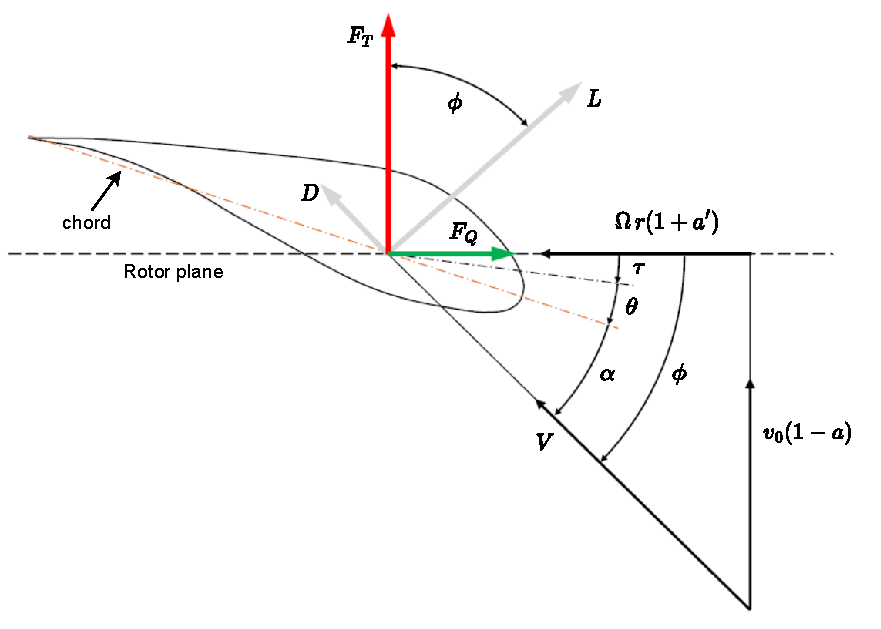
\includegraphics[width=.55\textwidth]{../Graphics/BladeVelocityTriangle.pdf}%
			\label{fig:blade_vel_triangle}}
		\label{fig:blade_triangles}
	\end{figure}
\end{frame}

%%%%%%%%%%%%%%%%%%

\begin{frame}{Theoretical Background}{Something}
	\begin{itemize}
		\item A text in a dotted list in the theoretical background
	\end{itemize}
\end{frame}

%%%%%%%%%%%%%%%%%%





%%%%%%%%%%%%%%%%%%
%\begin{frame}{Big header}{Smaller header}
%	\textbf{Some text}
%	\begin{itemize}
%		\item Item
%	\end{itemize}
%\end{frame}
%


\section{Modelling}
\begin{frame}{Modelling}{Introduction}
	\begin{itemize}
		\item Dynamics relevant to fore-aft motion included
		\item First principles modelling
		\item Component modelled individually
		\item Only fore-aft motion model included in presentation
	\end{itemize}
\end{frame}

%%%%%%%%%%%%%%%%

\begin{frame}{Modelling}{Tower fore-aft motion}
	\begin{equation}
		\begin{split}
			\dot{v}_y & = \dfrac{F_{rot} - b v_y - k p_y}{m} \\
			\dot{p}_y & = v_y
		\end{split}
	\end{equation}
	\begin{equation}
			k = (2 \pi f_{eig})^2 m \;\; , \;\; b = 2 \zeta \sqrt{k m}
	\end{equation}
	\begin{figure}[ht]
		\centering
		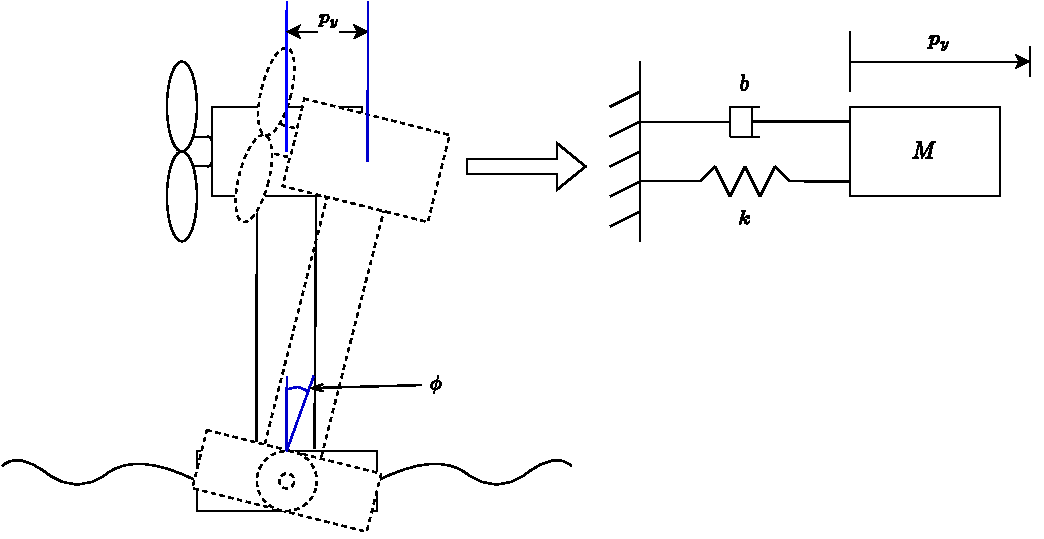
\includegraphics[width=0.9\linewidth]{../Graphics/wtLinForeAftMotionModel.pdf}
		\label{fig:wtLin_fore-aft_diagram}
	\end{figure}
\end{frame}

%%%%%%%%%%%%%%%%

\begin{frame}{Modelling}{Fore-aft model fitting}
	Fore-aft motion model parameter fitting results:
	\begin{columns}
		\begin{column}{.49\textwidth}
			\begin{figure}[ht]
				\centering
				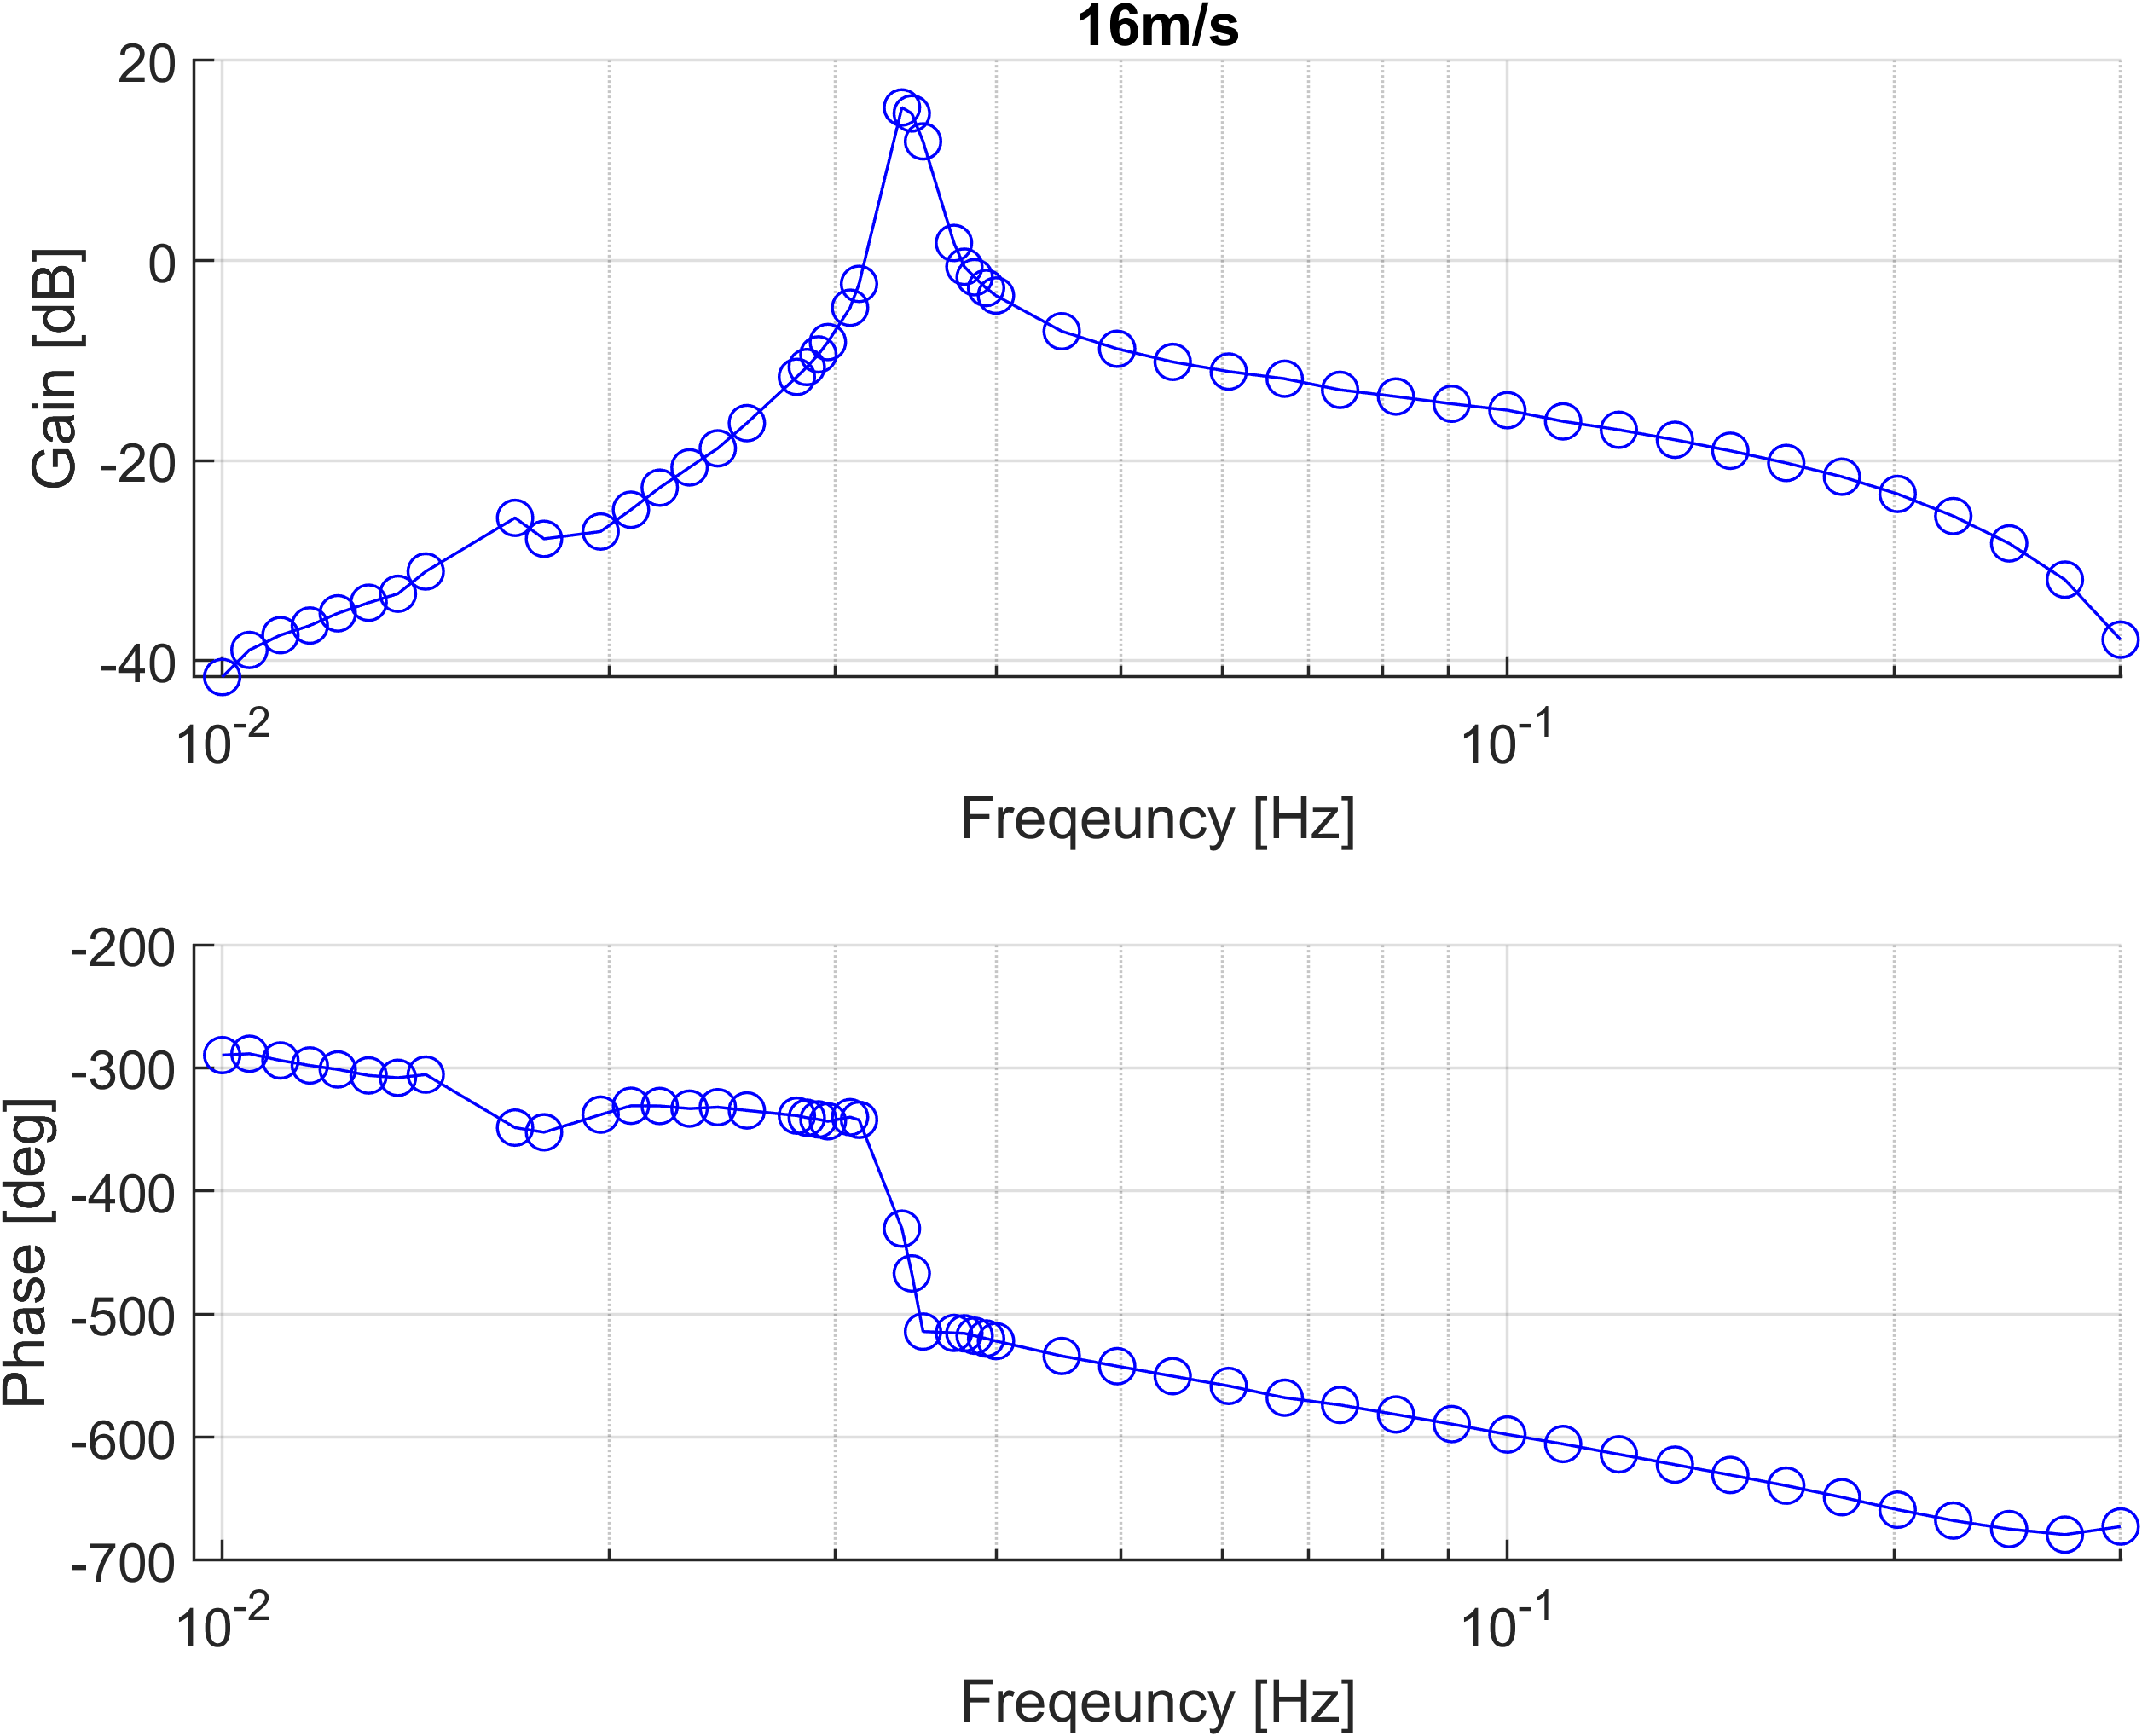
\includegraphics[width=1\linewidth]{../Graphics/TestResults/foreaftFitting/sysid_thSine-vy_16ms.png}
				\label{fig:sysid_wref-vy_16}
			\end{figure}
			\centering VTS
		\end{column}
	
		\begin{column}{.49\textwidth}
			\begin{figure}[ht]
				\centering
				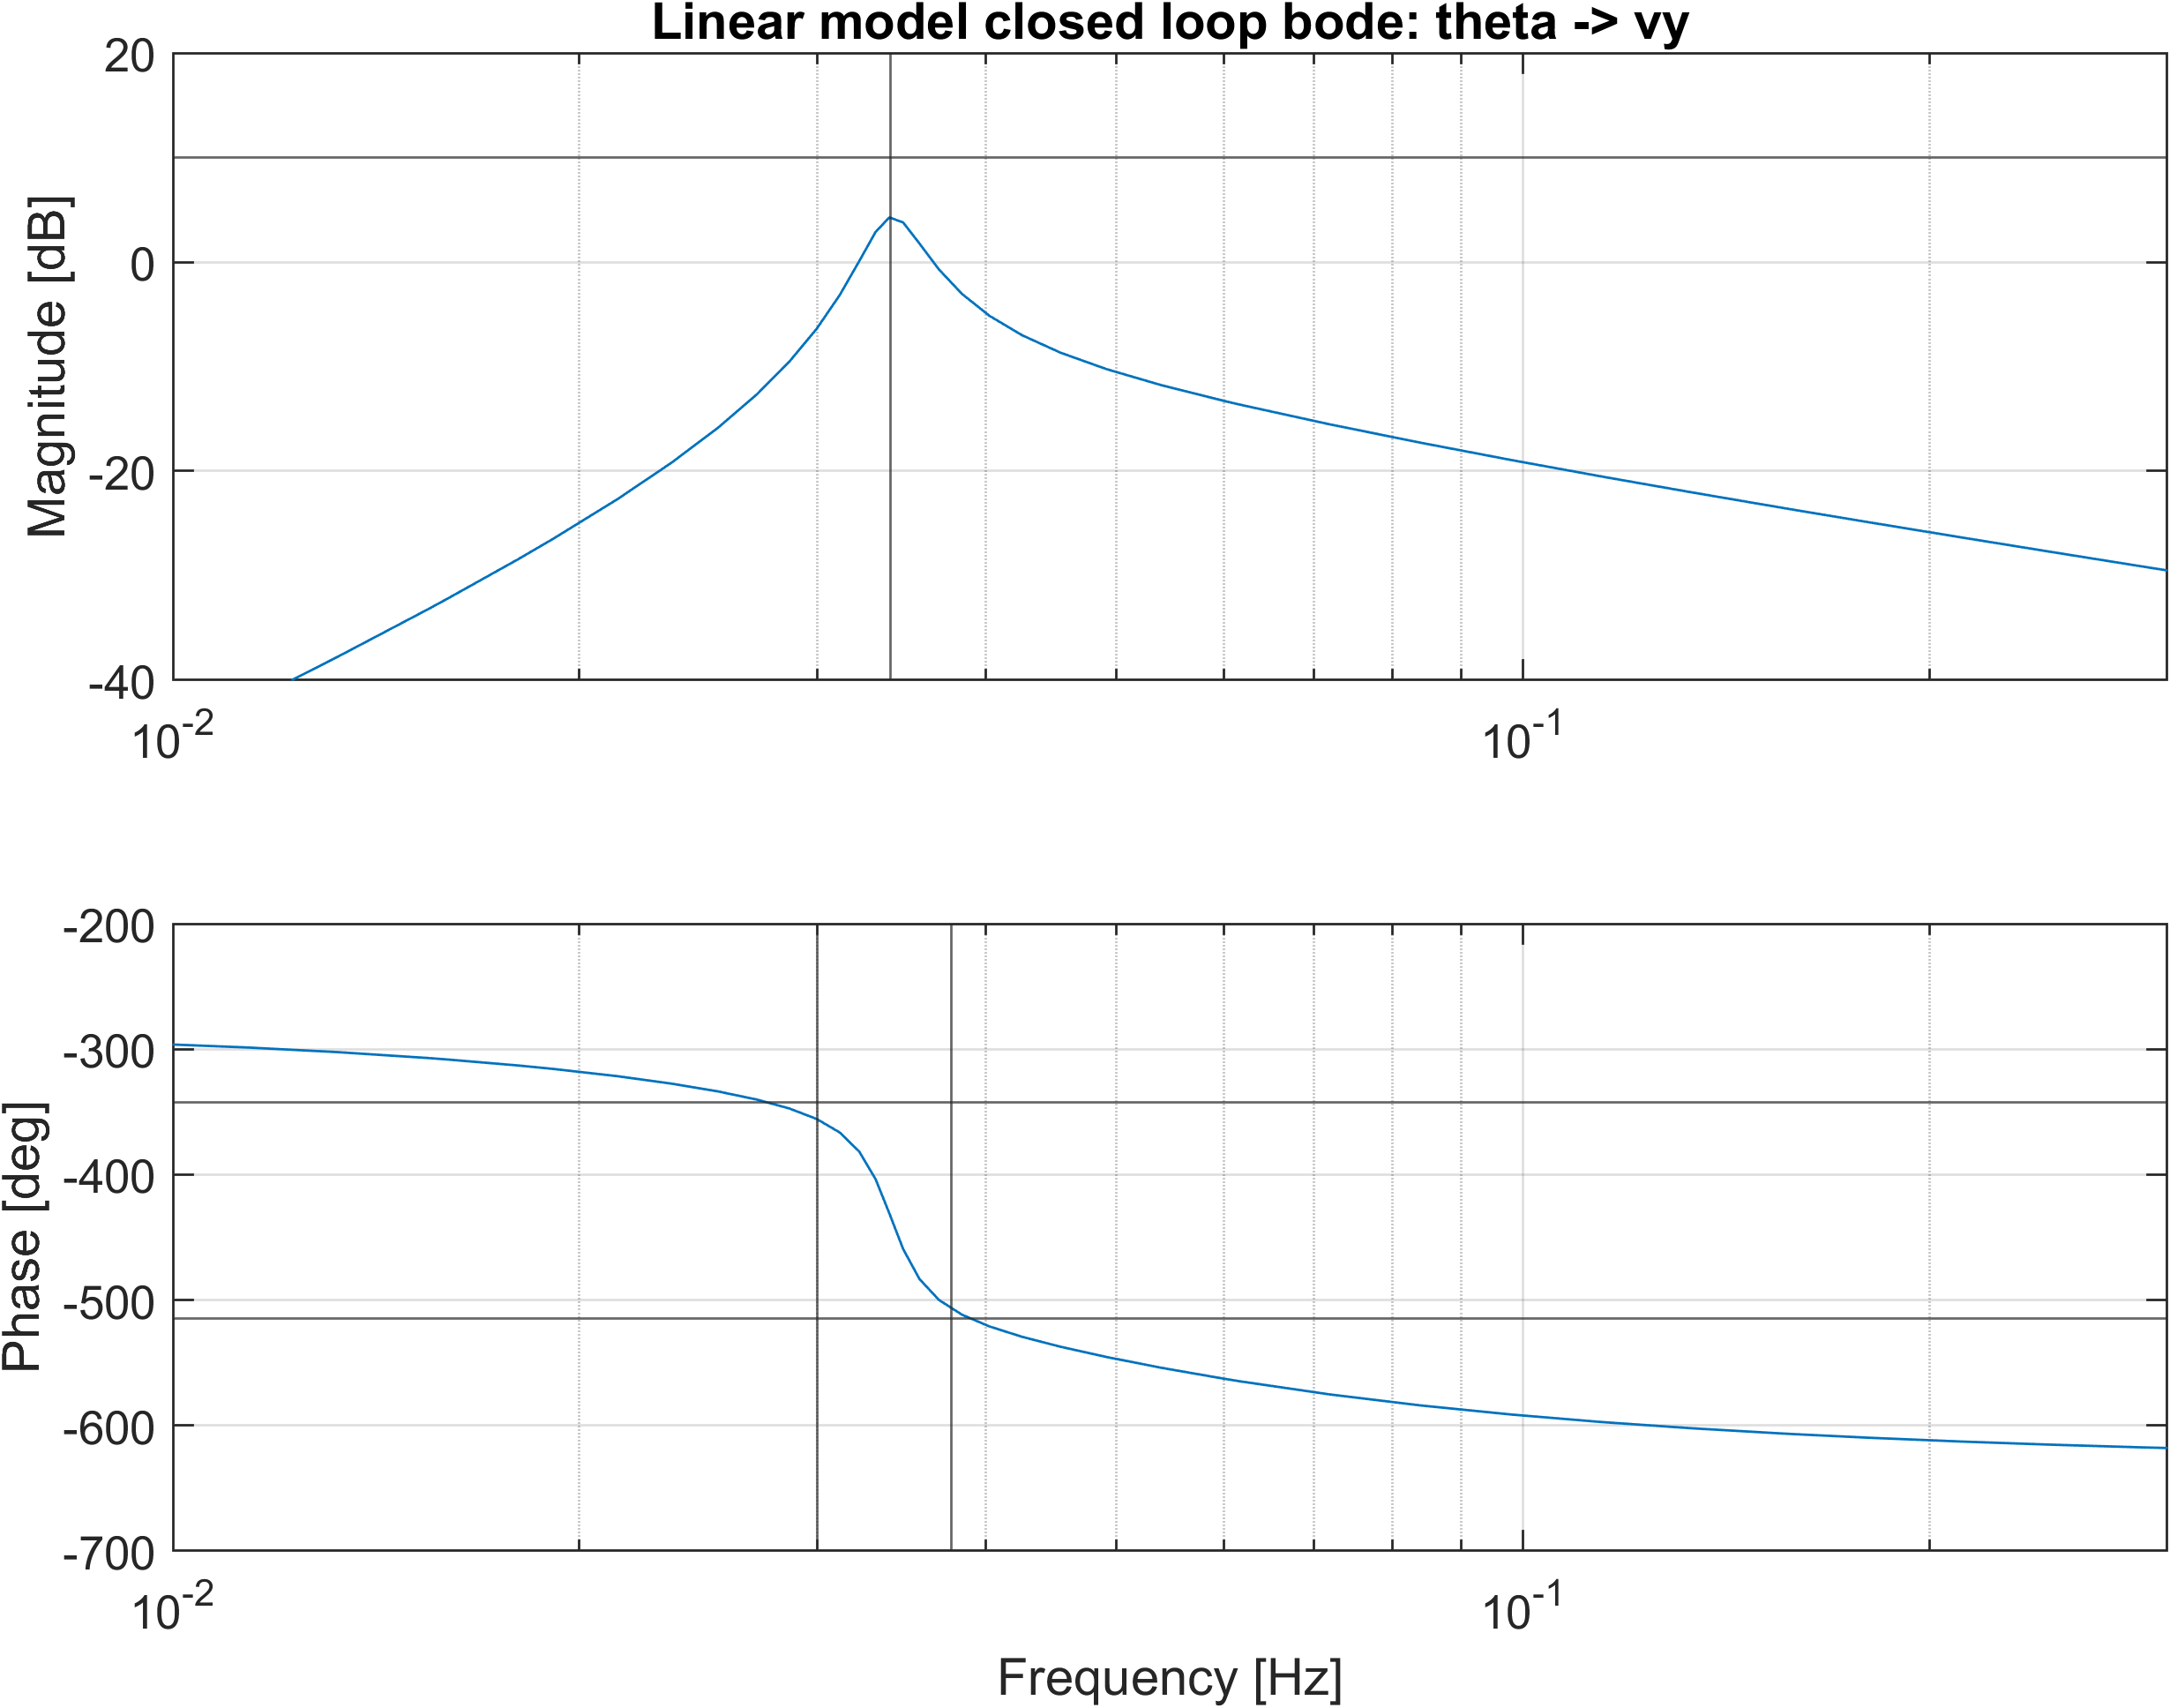
\includegraphics[width=1\linewidth]{../Graphics/TestResults/foreaftFitting/wtLin_th-vy_16ms.png}
				\label{fig:wtlin_wref-vy_16}
			\end{figure}
			\centering Linear model
		\end{column}
	\end{columns}
	
\end{frame}

%%%%%%%%%%%%%%%%

\begin{frame}{Modelling}{The model}
	The resulting state-space model:
	\begin{itemize}
		\item \textbf{States:} \{$ p_y, v_y, \Omega, \Omega_{int} $\} \hspace{1mm} with $ \Omega =$ rotor speed
		\item \textbf{Input:} \{$ \omega_{ref} $\} \hspace{1mm} with $ \omega =$ generator speed
		\item \textbf{Disturbance:} \{$ v_{free} $\}
		\item \textbf{Outputs:} \{$ p_y, v_y, \Omega $\}
		\item Stable
		\item Controllable and observable
	\end{itemize}	
\end{frame}

\section{Controller Design}
\begin{frame}{Controller Design}{Infinite-Horizon Linear-Quadratic Regulator}
	\begin{equation}\label{eq:lqr_cost}
		J = \int_{0}^{\infty} \left(x^T Q x + u^T R u + 2x^T N u\right) dt
	\end{equation}
	where
	\begin{center}
		\begin{tabular}{l r l }
			weight & $R$         & $ > 0$\hspace{1mm} (positive definite) and symmetric       \\
			weight & $Q$		 & $\ge 0$\hspace{1mm} (positive semi-definite) and symmetric
		\end{tabular}
	\end{center}
	Controller gain
	\begin{equation}\label{eq:lqr_K}
		K = -R^{-1} B^T P
	\end{equation}
	with P being the solution to the algebraic Ricatti equation:
	\begin{equation}\label{lqr:ricatti}
		A^T P + P A - P B R^{-1} B^T P + Q = 0
	\end{equation}
	Matlab: \textit{lqr(A, B, Q, R, N)}
	
	\smallskip
	Bryson's Rule:
	\begin{equation}\label{eq:bryson}
			Q_i = \dfrac{1}{Max(\hat x_i)^2} \;\; , \;\; R_i = \dfrac{1}{Max(\hat u_i)^2}
	\end{equation}
\end{frame}

%%%%%%%%%%%%%%%%

\begin{frame}{Controller Design}{Integral action}
	Integral action is necessary for proper rotor speed control. System is augmented with integral state:
	\begin{align} 
		\dot {\bar x} & = \begin{bmatrix} \dot{\hat x} \\ \dot x_i \end{bmatrix} = \begin{bmatrix} A &0 \\ C_{iy} & 0 \end{bmatrix} \bar x + \begin{bmatrix} B_u \\ 0 \end{bmatrix}  \hat u \\
		\bar y & = \begin{bmatrix} C & 0 \end{bmatrix} \bar x
	\end{align}
	$ C_{iy} $ picks out desired output for integration ($\Omega$)
	
	\begin{itemize}
		\item Integral state is included in LQR algorithm
		\item Weight on integral state is awkward place
	\end{itemize}
\end{frame}


%%%%%%%%%%%%%%%%

%\begin{frame}{Controller Design}{Analysis of LQI controller poles}
%	It was of interest to see how closed-loop system poles moved when changing LQI $ Q $ and $ R $ weights.
%	\begin{itemize}
%		\item A text
%	\end{itemize}\bigskip
%\end{frame}

\section{Test Results}
\begin{frame}{Test Results}{Linear model}
	\begin{itemize}
		\item A text
	\end{itemize}
\end{frame}

%%%%%%%%%%%%%%%%

\begin{frame}{Test Results}{VTS: 16 m/s}
	\begin{itemize}
		\item A text
	\end{itemize}\bigskip
\end{frame}


%%%%%%%%%%%%%%%%

\begin{frame}{Test Results}{VTS: 16 m/s}
	\begin{itemize}
		\item A text
	\end{itemize}\bigskip
\end{frame}


%%%%%%%%%%%%%%%%

\begin{frame}{Test Results}{VTS: 12 \& 26 m/s m/s}
	\begin{itemize}
		\item A text
	\end{itemize}\bigskip
\end{frame}


%%%%%%%%%%%%%%%%

\begin{frame}{Test Results}{VTS: 12 \& 26 m/s m/s}
	\begin{itemize}
		\item A text
	\end{itemize}\bigskip
\end{frame}

\section{Conclusion}
\begin{frame}{Conclusion}{}
	\begin{itemize}
		\item A simple linear model was proven to sufficiently capture the the fore-aft motion dynamics.
		\item A simple mass-spring-damper model successfully modelled the fore-aft motion
		\item The developed LQI controller developed achieved rotor speed tracking with zero steady state error and fore-aft motion damping
		\item In VTS implementation: Real states of position and velocity are fed to controller
		\item Deviation observed between linear model and VTS behaviour with fixed-bottom FLC
		\item LQI controller successfully implemented in VTS and achieved satisfactory rotor speed tracking while greatly damping fore-aft motion
		\begin{itemize}
			\item Bryson's rule
			\item LQI had slightly higher actuator activity than detuned FLC
			\item Superior to fixed-bottom FLC and the detuned FLC
		\end{itemize}
	\item LQI controller parameters recalculation for other OPs partly or fully improves performance
	\end{itemize}
\end{frame}








% ======================================================================




%\section{References}
%\begin{frame}{References}
%	\bibliographystyle{ieeetran}
%	\bibliography{../../RefLib/CA7Projekt.bib}
%\end{frame}

{\aauwavesbg
\begin{frame}[plain,noframenumbering]
  \finalpage{Open for questions}
\end{frame}}
%%%%%%%%%%%%%%%%

\end{document}
